%%%%%%%%%%%%%%%%%%%%%%%%%%%%%%%%%%%%%%%%%
% Long Lined Cover Letter
% LaTeX Template
% Version 1.0 (1/6/13)
%
% This template has been downloaded from:
% http://www.LaTeXTemplates.com
%
% Original author:
% Matthew J. Miller
% http://www.matthewjmiller.net/howtos/customized-cover-letter-scripts/
%
% License:
% CC BY-NC-SA 3.0 (http://creativecommons.org/licenses/by-nc-sa/3.0/)
%
%%%%%%%%%%%%%%%%%%%%%%%%%%%%%%%%%%%%%%%%%

%----------------------------------------------------------------------------------------
%	PACKAGES AND OTHER DOCUMENT CONFIGURATIONS
%----------------------------------------------------------------------------------------

\documentclass[5pt,stdletter,dateno,sigleft]{newlfm} % Extra options: 'sigleft' for a left-aligned signature, 'stdletternofrom' to remove the from address, 'letterpaper' for US letter paper - consult the newlfm class manual for more options

\usepackage{charter} % Use the Charter font for the document text
\usepackage{hyperref}
\hypersetup{
%draft, % Uncomment to remove all links (useful for printing in black and white)
colorlinks=true, breaklinks=true, bookmarks=true,bookmarksnumbered,
urlcolor=blue, linkcolor=blue, citecolor=blue, % Link colors
pdftitle={}, % PDF title
pdfauthor={\textcopyright}, % PDF Author
pdfsubject={}, % PDF Subject
pdfkeywords={}, % PDF Keywords
pdfcreator={pdfLaTeX}, % PDF Creator
pdfproducer={LaTeX with hyperref and ClassicThesis} % PDF producer
}

\newsavebox{\Luiuc}\sbox{\Luiuc}{\parbox[b]{1.75in}{\vspace{0.4in}
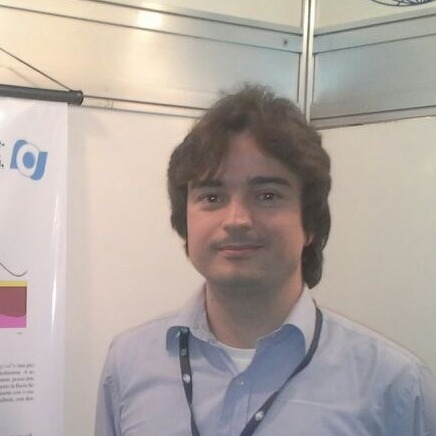
\includegraphics[width=0.7\linewidth]{logo.jpg}}} % Company/institution logo at the top left of the page
\makeletterhead{Uiuc}{\Lheader{\usebox{\Luiuc}}}

\newlfmP{sigsize=25pt} % Slightly decrease the height of the signature field
\newlfmP{addrfromphone} % Print a phone number under the sender's address
\newlfmP{addrfromemail} % Print an email address under the sender's address
\PhrPhone{Phone} % Customize the "Telephone" text
\PhrEmail{Email} % Customize the "E-mail" text


\lthUiuc % Print the company/institution logo

%----------------------------------------------------------------------------------------
%	YOUR NAME AND CONTACT INFORMATION
%----------------------------------------------------------------------------------------

\namefrom{Victor Ribeiro Carreira} % Name

\addrfrom{
\today\\[12pt] % Date
37 Manuel Magioli Street  \\ % Address
Rio de Janeiro, Rio de Janeiro 21940-270
}

\phonefrom{(55+21) 99828-8484 \\ Skype: carreira,v.r.} % Phone number

\emailfrom{carreiravr@gmail.com} % Email address


%----------------------------------------------------------------------------------------
%	ADDRESSEE AND GREETING/CLOSING
%----------------------------------------------------------------------------------------

\greetto{To Whom it may concern,} % Greeting text
\closeline{Sincerely yours,} % Closing text

\nameto{Lagesed} % Addressee of the letter above the to address

\addrto{
Open Jobs Positions \\ % To address
Universidade Federal do Rio de Janejro-UFRJ, Geology Department \\
}

%----------------------------------------------------------------------------------------

\begin{document}
\begin{newlfm}

%----------------------------------------------------------------------------------------
%	LETTER CONTENT
%----------------------------------------------------------------------------------------

The reason for writing this letter is that I would like to be considered for a position in Lagesed rock descripitive job. I have learned about this career opportunities at web and with friends that already work in the laboratory (\href{http://lagesed.geologia.ufrj.br/presal-bacia-de-santos/}{Lagesed job reference})

%PARAGRAPH ONE: State the reason for the letter, name the position or type of work you are applying for and identify the source from which you learned of the opening (i.e. career development center, newspaper, employment service, personal contact).

I am a master certificated student and now I am doing my PhD and I develop new tools for well logging analysis and geological description. My main role in the area, in geophysics, is related to creation of models for sedimentary basins. In my master's work I have created interpreted a model of a 2D section of the Parana Intracratonic Sedimentary Basin using an innovative methodology with geological correlation. In the process, I have to learn and use programming language such as python, fortran 95, Octave, among others (\href{https://github.com/VictorCarreira}{Program learning skills}). Now I also include Pandas package that is directly related to Data Base area (one of the requirements for the jog description). In my PhD I have created a program that relates physical data performed by well logging with strings (rock description). 

I have, also, one year experience in geological field mapping and geophysical data acquisition as a field geology in National Observatory, Rio de Janeiro. I am interested in an institution that offers professional challenge and, above all, emphasis in continuous learning. In the case of Lagesed, these qualities apply. The chance to be part of such environment would be an incomparable experience. Furthermore, this partnership will be incredible helpfull in the second phase of my PhD. Some of my published work can be found at my online CV and my \href{https://www.researchgate.net/profile/Victor_Carreira}{published work's page}.

%PARAGRAPH TWO: Indicate why you are interested in the position, the company, its products, services - above all, stress what you can do for the employer. If you are a recent graduate, explain how your academic background makes you a qualified candidate for the position. If you have practical work experience, point out specific achievements or unique qualifications. Try not to repeat the same information the reader will find in the resume. Refer the reader to the enclosed resume or application which summarizes your qualifications, training, and experiences. The purpose of this section is to strengthen your resume by providing details which bring your experiences to life.

I welcome the opportunity to discuss this position with you further and look forward to hearing from you. I am turning myself available for interviews.

%PARAGRAPH THREE: Request a personal interview and indicate your flexibility as to the time and place. Repeat your phone number in the letter and offer assistance to help in a speedy response. For example, state that you will be in the city where the company is located on a certain date and would like to set up an interview. Alternatively, state that you will call on a certain date to set up an interview. End the letter by thanking the employer for taking time to consider your credentials.

Thank you very much for your time.

%----------------------------------------------------------------------------------------

\end{newlfm}
\end{document}
